



\labday{Web Server}
Here are some definitions to start:
\begin{itemize}
\item {\bf URI (Uniform Recsource Identifier}- The suffix of the corresponding URS that includes the filename and optional arguments.
\item {\bf Network Port}- A number signaling what different type of traffic is sent over (email, internet, texts).  Ports talk to other devices as well as other networks through these ports.  
\item {\bf Sockets}- Let the client and server talk over ports by providing an API that allows communication between the server and the client.  Sockets talk to applications.
\end{itemize}

\experiment{Protocol Layering}
A {\bf  protocol } is a set of layers used to communicate with eachother.  Each instance of a protocol talks virtually to its peer using the protocol.  Each instance of a protocol uses only the servicese of a lower layer.  Protocols must provide two things:
\begin{itemize}
\item Provides a naming scheme for host addresses, a unique address to identify itself.
\item Provide a delivery mechanism called a packet which consists of a header and a payload.  Header contains size, source, and destination.  Payload contains bits sent from source.
\end{itemize}


\begin{figure}[H] % Example of including images
\begin{center}
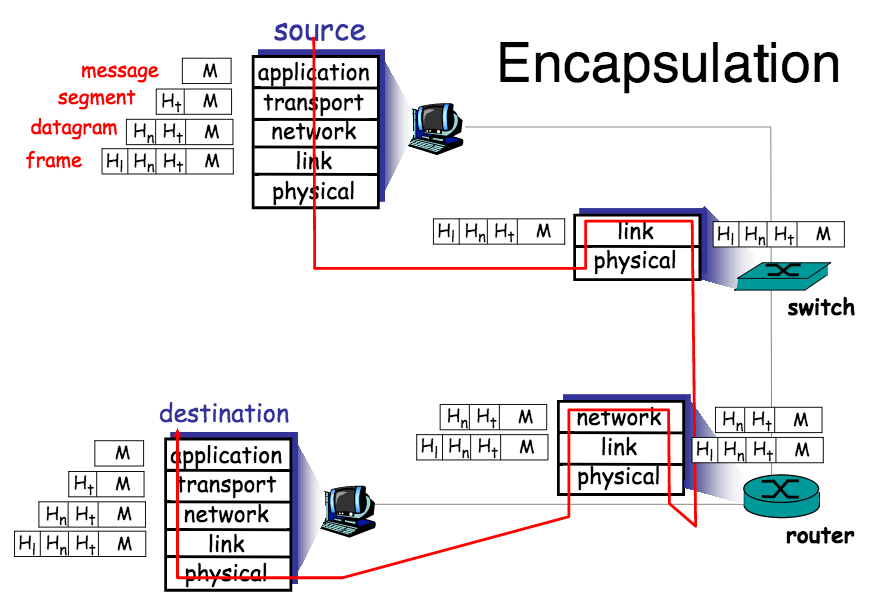
\includegraphics[width=.8\linewidth]{encapsulation}
\end{center}
\caption{How protocol layering works}
\label{fig:example_figure}
\end{figure}
